\section{Measurement Model}
We consider the problem of recovery of a signal from its modulo measurements obtained through compressive sensing. Simply put, we aim to recover $\mathbf{x^*}\in \R^n$ from the modulo measurements $y_i=\mod(\langle \mathbf{a_i} \cdot \mathbf{x^*} \rangle,R)$ for $i = \{1,2,...,m\}$, where $\mod$ is modulo operation with respect to a fixed, real-valued parameter $R$. Typically, $m<n$. For simplicity, we assume that the modulo function operates only within two periods, one each on the either side of the origin, as shown in the Fig.~\ref{fig:graph}. We construct $\mathbf{A} = \left[\mathbf{a_1~a_2~...~a_m}\right]^T$ with i.i.d. Gaussian entries. The primary assumption in our model is that the natural signal $\mathbf{x^*}$ is $s-$sparse in a chosen basis. 

\begin{figure}[h]
	\begin{center}
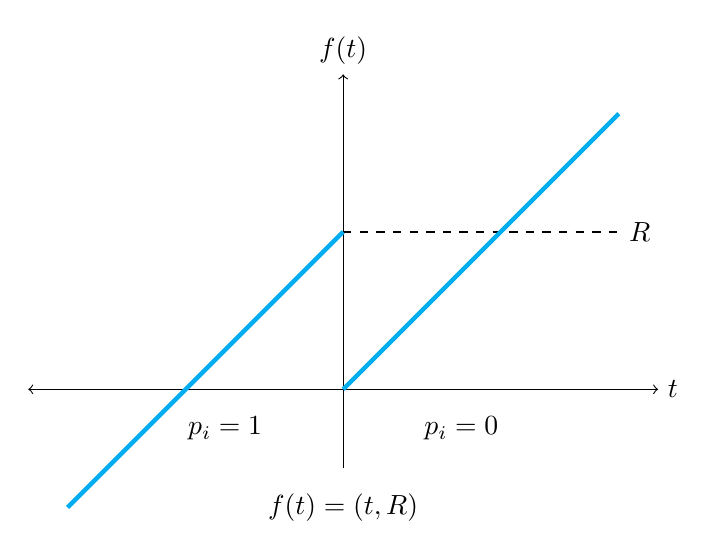
\begin{tikzpicture}
\draw[<->] (-4,0) -- (4,0) node[right] {$t$};
\draw[->] (0,-1) -- (0,4) node[above] {$f(t)$};
\draw[scale=0.5, dashed, thick] (0,4)--(7,4) node[right]{$R$};
\draw (1.5,-0.5) node(below) {$p_i = 0$};
\draw (-1.5,-0.5) node(below) {$p_i = 1$};
\draw (0,-1.5) node(right) {$f(t) = \mod(t,R)$};
\draw[scale=0.5,domain=-7:0,smooth,variable=\x,cyan, ultra thick] plot ({\x},{\x+4});
\draw[scale=0.5,domain=0:7,smooth,variable=\x,cyan, ultra thick]  plot ({\x},{\x});
\end{tikzpicture}
\end{center}
\caption{\emph{Modified modulo function for the given problem}}
\label{fig:graph}
\end{figure}

We can write the modified equation for the modulo operation under consideration as:
$$
f(t) = \mod(t,R) = t+\left( \frac{1-\sgn(t)}{2}\right)R,
$$
where $\sgn(t)$ is a signum function.

For the measurement model of the given problem, 
We define the corrected linear measurements as: 

$$
y_{c,i} =\langle \mathbf{a_i} \cdot \mathbf{x^*} \rangle.
$$

We also define each element of the true bin-index vector $\mb{p^*}$ as,
$$
p^*_i = \frac{1-\sgn(\langle \mathbf{a_i} \cdot \mathbf{x^*} \rangle)}{2}.
$$
Thus,
$$
y_i = \langle \mathbf{a_i} \cdot \mathbf{x^*} \rangle + p^*_iR = y_{c,i}+p^*_iR.
$$

It is evident that if we can recover $\mathbf{p^*}$ successfully, we can calculate the correct compressed measurements $\langle \mathbf{a_i} \cdot \mathbf{x^*} \rangle$ and use them to reconstruct $\mathbf{x^*}$ with any sparse recovery algorithm such as CoSaMP.


\section{Reconstruction Algorithm}

In this section, we describe our AltMin based approach to recover $\mathbf{x^*}$ and $\mathbf{p^*}$, given $\mathbf{y, A}, s, R$. We call our algorithm MoRAM - Modulo Reconstruction using Alternative Minimization. Our approach comprises of two steps: (i) initialization step, and (ii) Descent step through alternative minimization.

\subsection{Initialization using Re-Calculated Measurements (RCM)}
Similar to other non-convex approaches, MoRAM also requires an initial estimate $\mathbf{{x}^0}$ that is close to the true signal $\mathbf{{x}^*}$. We have several initialization techniques available, typically used in Phase Retrieval problems; such as spectral initialization. However, the nature of the problem in our case is fundamentally different due to asymmetric and non-linear behavior of the modulo transfer function. To overcome this issue, we propose a method to re-calculate the true measurements ($\mb{y_c}= \mb{Ax^*}$) from the available modulo measurements. We aim to undo the effect of modulo operation for the fraction of the total measurements. To understand the method for such re-calculation, we will first try to understand the effect of modulo operation on the linear measurements.

\subsubsection{Undo the effect of modulo operation} 

We observe the histograms of the $\mathbf{Ax^*}$(Fig.~\ref{fig:hist1}) and $\mathbf{\mod(\mathbf{Ax^*})}$(Fig.~\ref{fig:hist2}) to understand the information we can obtain from the modulo measurements. We are particularly interested in the case where signal strengths are low compared to the value of $R$, nevertheless, we also analyze the other case when $R$ is less than the signal strength. Here, we define $\rho$ as maximum element in $\mathbf{Ax^*}$. $\rho$ is bounded by a real number with very high probability, as the distribution of $\mathbf{Ax^*}$ is Gaussian.
In Fig.~\ref{fig:hist2} and Fig.~\ref{fig:hist3}, we can see the histogram after modulo operation for both the cases: $R>\rho$ and $R<\rho$. Comparing these histograms with the histogram of true measurements (Fig.~\ref{fig:hist1}), we can observe how the values of first histogram translates into second or third when the modulo operation is applied. We can draw following conclusions:
\begin{itemize}
	\item Only the values lying on the negative side of the x-axis are going to be affected.
	\item Values lying very close to the origin on the negative side of the x-axis in the first histogram, would now shift by $R$, and would occupy a place very close to $R$ in second histogram. For $R>\rho$, this region is shaded with green color in Fig.~\ref{fig:hist2}. Correct bin-value for the elements in $\mathbf{y}$ with value lying between $\rho$ and $R$ is $p_{rcm,i} = 1$.
	\item For $R>\rho$, histogram of the positive region very close to the origin would remain unaffected. This region is shaded with orange color in Fig.~\ref{fig:hist2}. Correct bin-value for all the elements in $\mathbf{y}$ with value lying between $0$ and $R-\rho$ is $p_{rcm,i} = 0$.
	\item Nothing can be concluded for measurements lying in between the above mentioned ranges. This region is shaded with gray color in Fig.~\ref{fig:hist2} and Fig.~\ref{fig:hist3}. Correct bin-value cannot be identified for this region, so we assign all the elements in $\mathbf{y}$ with value lying between $0$ and $(R-\rho)$ as $p_{rcm,i} = 0$. The lower and upper bounds ($t_l \& t_u$) of this disputed region can be obtained as, 
	$$t_l = \max(0, R-\rho)$$
	$$t_u = \max(\rho, R)$$.
	\item Irrespective of relationship between $\rho$ and $R$, all the values lying in the negative half of the real line have the bin-value equal to $1$, and all the values greater than $R$ have the bin-value equal to $0$.
\end{itemize}

\begin{algorithm}[t]
	\caption{\textsc{RCM-Initialization}}
	\label{alg:RCM}
	\begin{algorithmic}
		\State\textbf{Inputs:} $\mathbf{y}$, $\mathbf{A}$, $s$, $R$, $\rho$
		\State\textbf{Output:}  $\mb{x^0}$
		\State $T \leftarrow \phi$, $t_l \leftarrow \max(0, R-\rho)$, $t_u \leftarrow \max(\rho, R)$
		\For {$l= 0:m$}
		\If {$y_l<0$}
		\State {$p^rcm_l = 1$, $T \leftarrow T \cup {l}$}
		\ElsIf {$0\leq y_l < t_l$}
		\State {$p^rcm_l = 0$, $T \leftarrow T \cup {l}$}
		\ElsIf {$t_l\leq y_l < t_u$}
		\State {$p^rcm_l = 0$}
		\ElsIf {$t_u \leq y_l < R$}
		\State {$p^rcm_l = 1$, $T \leftarrow T \cup {l}$}
		\ElsIf {$R  \leq y_l$}
		\State {$p^rcm_l = 0$, $T \leftarrow T \cup {l}$}
		
		\EndIf	
		\EndFor
		\State $N \leftarrow |T|$
		\State $\mb{x^0} \leftarrow H_s\left( \frac{1}{N}\sum_{i=1}^{N}y_{T,i}a_{T,i}\right)$
	\end{algorithmic}
\end{algorithm}




\begin{figure}[h]
	\begin{center}
		\begin{tikzpicture}
		\def\normaltwo{\x,{3*1/exp(((\x)^2)/2)}}
		\def\y{4.4}
		
		%\fill [fill=orange!60] (2.6,0) -- plot[domain=0:4.4] (\normaltwo) -- ({\y},0) -- cycle;
		
		% Draw and label normal distribution function
		\draw[color=blue,domain=-3:3,thick] plot (\normaltwo) node[right] {};
		\draw[<->] (-5,0) -- (5,0) node[right] {$\mathbf{Ax^*}$};
		\draw[<->] (0,-1) -- (0,4);
		
		\draw (-3,-0.5) node(below) {$-\rho$};
		\draw (-4,-0.5) node(below) {$-R$};
		\draw (3,-0.5) node(below) {$\rho$};
		\draw (4,-0.5) node(below) {$R$};
		
		\foreach \x in {-3,-4,3,4}
		{        
			\coordinate (A\x) at ($(0,0)+(\x*1cm,0)$) {};
			\draw ($(A\x)+(0,5pt)$) -- ($(A\x)-(0,5pt)$);
			
		}
		%		\draw (-1.5,-0.5) node(below) {$p_i = 1$};
		%		\draw (0,-1.5) node(right) {$f(t) = \mod(t,R)$};
		%		\draw[scale=0.5,domain=-7:0,smooth,variable=\x,cyan, ultra thick] plot ({\x},{\x+4});
		%		\draw[scale=0.5,domain=0:7,smooth,variable=\x,cyan, ultra thick]  plot ({\x},{\x});
		\end{tikzpicture}
	\end{center}
	\caption{\emph{Histogram of $\mathbf{Ax^*}$}}
	\label{fig:hist1}
\end{figure}
\begin{figure}[h]
	\begin{center}
		\begin{tikzpicture}
		\def\normaltwo{\x,{3*1/exp(((\x)^2)/2)}}
		\def\normalone{\x,{3*1/exp(((\x-4)^2)/2)}}
		\def\normalsum{\x,{3*1/exp(((\x-4)^2)/2)+3*1/exp(((\x)^2)/2)}}
		\def\y{3}
		\def\fy{3*1/exp(((\y-4)^2)/2)}
		\fill [fill=orange!60] (0,0) -- plot[domain=0:1] (\normaltwo) -- (1,0) -- cycle;
		\fill [fill=green!60] (3,0) -- plot[domain=3:4] (\normalone) -- (4,0) -- cycle;
		\fill [fill=gray!30] (1,0) -- plot[domain=1:3] (\normalsum) -- (3,0) -- cycle;
		% Draw and label normal distribution function
		\draw[color=blue,domain=-0:3,dashed,thick] plot (\normaltwo) node[right] {};
		\draw[color=blue,domain=1:4,dashed,thick] plot (\normalone) node[right] {};
		\draw[color=blue,domain=-0:4,thick] plot (\normalsum) node[right] {};
		\draw[<->] (-5,0) -- (5,0) node[right] {$\mathbf{Ax^*}$};
		\draw[<->] (0,-1) -- (0,4);
		\draw[dashed] ({\y},{\fy}) -- ({\y},0);
		\draw[dashed] ({4},{3}) -- ({4},0);
		\draw[dashed] ({1},{\fy}) -- ({1},0);
		\draw (-3,-0.5) node(below) {$-\rho$};
		\draw (-4,-0.5) node(below) {$-R$};
		\draw (3,-0.5) node(below) {$\rho$};
		\draw (4,-0.5) node(below) {$R$};
		\draw (1,-0.5) node(below) {$R-\rho$};
		\draw (0.5,1) node(below) {$p_i=0$};
		\draw (3.5,1) node(below) {$p_i=1$};
		\draw (2,0.5) node(below) {$p_i=0$};
		\foreach \x in {-3,-4,1,3,4}
		{        
			\coordinate (A\x) at ($(0,0)+(\x*1cm,0)$) {};
			\draw ($(A\x)+(0,5pt)$) -- ($(A\x)-(0,5pt)$);
			
		}
		%		\draw (-1.5,-0.5) node(below) {$p_i = 1$};
		%		\draw (0,-1.5) node(right) {$f(t) = \mod(t,R)$};
		%		\draw[scale=0.5,domain=-7:0,smooth,variable=\x,cyan, ultra thick] plot ({\x},{\x+4});
		%		\draw[scale=0.5,domain=0:7,smooth,variable=\x,cyan, ultra thick]  plot ({\x},{\x});
		\end{tikzpicture}
	\end{center}
	\caption{\emph{Histogram of $\mod(\mathbf{Ax^*})$, $R>\rho$}}
	\label{fig:hist2}
\end{figure}

\begin{figure}[!h]
	\begin{center}
		\begin{tikzpicture}
		\def\normaltwo{\x,{3*1/exp(((\x)^2)/2)}}
		\def\normalone{\x,{3*1/exp(((\x-2)^2)/2)}}
		\def\normalsum{\x,{3*1/exp(((\x-2)^2)/2)+3*1/exp(((\x)^2)/2)}}
		\def\y{3}
		\def\fy{3*1/exp(((\y-4)^2)/2)}
		\fill [fill=orange!60] (-1,0) -- plot[domain=-1:0] (\normalone) -- (0,0) -- cycle;
		\fill [fill=green!60] (2,0) -- plot[domain=2:3] (\normaltwo) -- (3,0) -- cycle;
		\fill [fill=gray!30] (0,0) -- plot[domain=0:2] (\normalsum) -- (2,0) -- cycle;
		% Draw and label normal distribution function
		\draw[color=blue,domain=-0:3,dashed,thick] plot (\normaltwo) node[right] {};
		\draw[color=blue,domain=-1:2,dashed,thick] plot (\normalone) node[right] {};
		\draw[color=blue,domain=-0:2,thick] plot (\normalsum) node[right] {};
		\draw[<->] (-5,0) -- (5,0) node[right] {$\mathbf{Ax^*}$};
		\draw[<->] (0,-1) -- (0,4);
		%\draw[dashed] ({\y},{\fy}) -- ({\y},0);
		\draw[dashed] ({-1},{2}) -- ({-1},0);
		\draw[dashed] ({3},{2}) -- ({3},0);
		%\draw[dashed] ({1},{\fy}) -- ({1},0);
		\draw (-3,-0.5) node(below) {$-\rho$};
		\draw (-2,-0.5) node(below) {$-R$};
		\draw (3,-0.5) node(below) {$\rho$};
		\draw (2,-0.5) node(below) {$R$};
		\draw (-1,-0.5) node(below) {$-\rho+R$};
		\draw (-0.5,1) node(below) {$p_i=0$};
		\draw (2.5,1) node(below) {$p_i=1$};
		\draw (1,0.5) node(below) {$p_i=0$};
		\foreach \x in {-3,-2,-1,3,2}
		{        
			\coordinate (A\x) at ($(0,0)+(\x*1cm,0)$) {};
			\draw ($(A\x)+(0,5pt)$) -- ($(A\x)-(0,5pt)$);
			
		}
		%		\draw (-1.5,-0.5) node(below) {$p_i = 1$};
		%		\draw (0,-1.5) node(right) {$f(t) = \mod(t,R)$};
		%		\draw[scale=0.5,domain=-7:0,smooth,variable=\x,cyan, ultra thick] plot ({\x},{\x+4});
		%		\draw[scale=0.5,domain=0:7,smooth,variable=\x,cyan, ultra thick]  plot ({\x},{\x});
		\end{tikzpicture}
	\end{center}
	\caption{\emph{Histogram of $\mod(\mathbf{Ax^*})$, $R<\rho$}}
	\label{fig:hist3}
\end{figure}
We divide the number line in the following 5 intervals, and assign the bin-value accordingly:
\begin{equation}
{p}^rcm_{i} = 
\begin{cases}
1,& \text{if } y_i <0 \\
0,& \text{if } 0\leq y_i < t_l \\
0,& \text{if } t_l\leq y_i < t_u ~~~~ \textnormal{(region of uncertainity)} \\
1,& \text{if } t_u \leq y_i < R \\
0,& \text{if } R  \leq y_i. \\
\end{cases}
\label{eq:rcm}
\end{equation}
Thus, we can identify the correct bin values for part of the measurements just by observing their magnitude. We define set $T$ as the set of measurements for which we can identify the bin-values correctly. We introduce $N=:|T|$.
$$N = m - \textnormal{number of measurements lying in the region of uncertainity}$$
Value of $N$ largely depends on the difference between $\rho$ and $R$.

Once we identify the correct bin-values for part of the measurements, we can re-calculate corrected measurements as,
$$
\mathbf{y_{c} = y + p^rcmR}.
$$
We use these corrected measurements $\mathbf{y_{rcm}}$ to calculate the initial estimate $\mathbf{{x}^0}$ using the estimation step described in the upcoming section.

\subsubsection{Calculating the initial estimate from the corrected measurements}
In the estimation step, $\mb{x^0}$ is calculated only from the $N$ corrected measurements using first order unbiased estimator. For that, we use the versions of $\mb{y}$ and $A$ truncated to the indices belong to set $T$:
\begin{equation}
\mb{x^0} = H_s\left( \frac{1}{N}\sum_{i=1}^{N}y_{T,i}a_{T,i}\right)
\label{eq:init}
\end{equation}
where $H_s$ denotes the hard thresholding operator that keeps the $s$ largest absolute entries of a vector and sets the other entries to zero.

\subsection{Alternative Minimization}
\label{sec:altmin}
\begin{algorithm}[H]
	\caption{\textsc{MoRAM}}
	\label{alg:MoRAM}
	\begin{algorithmic}
		\State\textbf{Inputs:} $\mathbf{y}$, $\mathbf{A}$, $s$, $R$
		\State\textbf{Output:}  $\widehat{x}$
		\State $m,n \leftarrow \mathrm{size}(\mathbf{A})$ 
		\State \textbf{Initialization}
		\State $\mathbf{x^0} \leftarrow \textrm{RCM}(\mathbf{y, A})$ 
		\State \textbf{Alternative Minimization}
		\For {$l =0:\mathrm{max_iter}$}
		\State $\mathbf{{p}^{t}} \leftarrow \frac{\mathbf{1}-\sgn(\langle \mathbf{A} \cdot \mathbf{x^t} \rangle)}{2}$
		\State $\mathbf{y^t_c} \leftarrow \mathbf{y} - \mathbf{p^t}R$
		\State $\mathbf{{x}^{t+1}}\leftarrow \argmin_{\mb{u}=[\mathbf{x~d}]^T}\norm{u}_1 ~~ s.t.~ \begin{bmatrix} \mathbf{A} & \mathbf{I} \end{bmatrix}\mb{u} = \mathbf{y}.$ 
		\State $\implies \mathbf{{x}^{t+1}}\leftarrow JP(\frac{1}{\sqrt{m}}\begin{bmatrix} \mathbf{A} & \mathbf{I} \end{bmatrix},\frac{1}{\sqrt{m}}\mathbf{y},[\mathbf{x^t~~p^t}]^T)$.
		\EndFor
	\end{algorithmic}
\end{algorithm}


Using Eq.~\ref{eq:init}, we calculate the initial estimate of the signal $\mathbf{{x}^0}$ which is relatively close to the true vector $\mathbf{x^*}$. Starting with $\mathbf{{x}^0}$, we  calculate the estimates $\mathbf{p}$ and $\mathbf{x}$ in alternating fashion to converge to the original signal $\mathbf{x^*}$. At each iteration of our Alternative Minimization, we use the current estimate of the signal ${\mathbf{x^t}}$ to get the value of the bin-index vector $\mathbf{{p}^t}$ as following:
\begin{equation}
\mathbf{{p}^{t}} = \frac{\mathbf{1}-\sgn(\langle \mathbf{A} \cdot \mathbf{x^t} \rangle)}{2}.
\label{step1}
\end{equation}

 
 Given $\mathbf{x^0}$ is close to $\mathbf{x^*}$, $\mathbf{p^0}$ would also be close to $\mathbf{p^*}$. Ideal way is to calculate the correct compressed measurements $\mathbf{y^t_c}$ using $\mathbf{p^t}$, and use $\mathbf{y_c}$ with CoSaMP to calculate the next estimate $\mathbf{{x}_{t+1}}$. Thus,


$$
\mathbf{y^t_c} = \langle \mathbf{A}\mathbf{x^{t}} \rangle = \mathbf{y} - \mathbf{p^t}R,
$$
$$
\mathbf{{x}^{t+1}} = \argmin_{\mathbf{x} \in \mathcal{M}_s}\norm{\mathbf{Ax} - \mathbf{y^t_c}}_2^2, %~~\mathrm{s.to}~~x^* \in \mathcal{M}_s,
$$

\begin{equation}
\implies \mathbf{{x}^{t+1}} = \cosamp(\frac{1}{\sqrt{m}}\mathbf{A},\frac{1}{\sqrt{m}}\mathbf{y^t_c},s,\mathbf{x^t}).
\label{eq:cosamp}
\end{equation}


 However, it should be noted that even the small error $\mathbf{d} = \mathbf{p^t - p^*}$ would reflect heavily in the calculation of $\mathbf{y^t_c}$, as each incorrect bin-index would add a noise of the magnitude $R$ in $\mathbf{y^t_c}$. Experiments suggest that the CoSaMP is not robust enough to cope up with such large errors in $\mathbf{y^t_c}$. To tackle this issue, we augmented the sparse recovery problem using the fact that the nature of error $\mathbf{d^t_p}$ is sparse; and each erroneous element of $\mathbf{p}$ adds a noise of the magnitude $R$ in $\mathbf{y^t_c}$. We take the sparsity of $\mathbf{d^t}$ to be $s_p = 0.1\times m$, suggesting that at most the $10\%$ of the total elements are classified with wrong bin-indices.
 
 The augmented optimization problem becomes,
  
$$
\mathbf{{x}^{t+1}}=\argmin_{[\mathbf{x~d}]^T \in \mathcal{M}_{s+s_p}}\norm{\begin{bmatrix} \mathbf{A} & \mathbf{I} \end{bmatrix} \begin{bmatrix} \mathbf{x} \\ \mathbf{d} \end{bmatrix} - \mathbf{y^t_c}}_2^2, %~~\mathrm{s.to}~~x^* \in \mathcal{M}_s,
$$
\begin{equation}
\implies \mathbf{{x^{t+1}}} = \cosamp(\frac{1}{\sqrt{m}}\begin{bmatrix} \mathbf{A} & \mathbf{I} \end{bmatrix},\frac{1}{\sqrt{m}}\mathbf{y_c^t},s+s_p,[\mathbf{x^t~~p^t}]^T).
\label{eq:robcosamp}
\end{equation}
We call the step in Eq.~\ref{eq:robcosamp} a Robust CoSaMP. 
However, for using CoSaMP , it is required to specify the total sparsity value $(s +s_p)$, where $s_p$ is unknown. Thus, we employ Basis pursuit instead of CoSaMP, which doesn't rely on sparsity. The robust formulation of basis pursuit is referred as Justice Pursuit (JP) in the literature, specified in Eq.~\ref{eq:jp}.
\begin{equation}
\implies \mathbf{{x^{t+1}}} = JP(\frac{1}{\sqrt{m}}\begin{bmatrix} \mathbf{A} & \mathbf{I} \end{bmatrix},\frac{1}{\sqrt{m}}\mathbf{y^t_c},[\mathbf{x^t~~p^t}]^T).
\label{eq:jp}
\end{equation}
We repeat the steps of bin index calculation (as in Eq.~\ref{step1}) and sparse recovery (as in Eq.~\ref{eq:cosamp} or Eq.~\ref{eq:robcosamp} or Eq.~\ref{eq:jp}) alternatively for $\mathrm{N}$ iterations. While the sparse recovery with robust CoSaMP (Eq.~\ref{eq:robcosamp}) improves the reconstruction performance for large values of $R$ by making the sparse recovery step less susceptible to the errors, CoSaMP can also used in its original form (as in Eq.~\ref{eq:cosamp}) for lower values of $R$. Nevertheless, the best performing recovery algorithm uses Justice Pursuit, which is able to produce perfectly converging results, as described in experimental section.

Thus, we can have two variants of the MoRAM algorithm: (i)MoRAM with CoSaMP, (ii) MoRAM with robust CoSaMP, and (iii) MoRAM with Justice Pursuit. 

%$$
%\norm{\begin{bmatrix} \mathbf{A} & \mathbf{I} \end{bmatrix} \begin{bmatrix} \mathbf{x^*} \\ \mathbf{d} \end{bmatrix} - \mathbf{y}}_2^2.
%$$

%
